\documentclass[varwidth=true, border=2pt]{standalone}
\usepackage{tikz}
\usetikzlibrary{shapes, calc, shapes, arrows}
\usepackage{amsmath,amssymb}

\usepackage{xcolor}
\definecolor{xvectorcolor}{HTML}{77933C}

\begin{document}
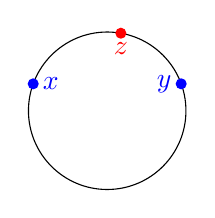
\begin{tikzpicture}
    \path (160:1) coordinate (X);
    \path ( 20:1) coordinate (Y);
    \path ( 80:1) coordinate (Z);

    \draw (0,0) circle (1);

    \fill[color=blue] (X) circle (2pt);
    \draw[blue] (X) node [right] {$x$};

    \fill[color=blue] (Y) circle (2pt);
    \draw[blue] (Y) node [left] {$y$};

    \fill[color=red] (Z) circle (2pt);
    \draw[red] (Z) node [below] {$z$};
\end{tikzpicture}
\end{document}
